%
% phi.tex
%
% (c) 2024 Prof Dr Andreas Müller
%
\begin{figure}
\centering
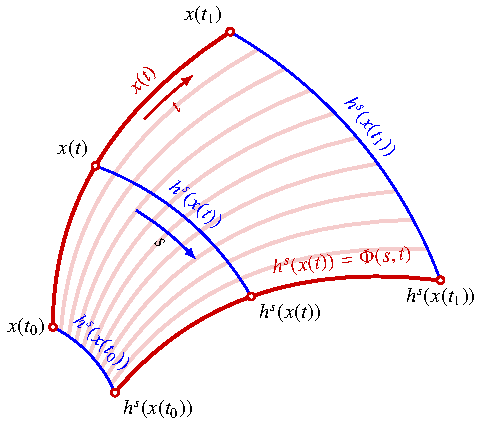
\includegraphics{chapters/100-symmetrien/images/phi.pdf}
\caption{Die Symmetrietransformation einer Bahnkurve $x(t)$ mit einer
differenzierbaren Symmetrietransformation $h^s$ ergibt eine Funktion von
zwei Variablen $\Phi(s,t)=h^s(x(t))$, die zum Beweis des Satzes von
Emmy Noether verwendet wird.
\label{buch:symmetrien:noether:fig:phi}}
\end{figure}
